Image generation forms an unsupervised learning task and therefore does not require labeled data.
The same applies for image compression.
Thus, any kind of image data can potentially be used for training and testing.

It is important to note that for conditional image generation, characterized by some guiding input like a class or
style that is supposed to be included in the generated image, labels can be of importance.
This does apply in our case, since in the paper, the \ac{vq} is used to generate images from specific classes.

Overall, the image generation and reconstruction performance of a model is highly dependent on the quality and diversity
of the training data.

\subsection{Feature Extraction}\label{subsec:feature-extraction}
In machine learning, a set of features is ``good'' if it allows the model to achieve a certain task
efficiently.
For traditional, non-deep models, that means that features should aim to be informative, meaning that
they should have some predictive value towards the final goal.
In simple regression settings, this is the case if the feature correlates with the true value.
Furthermore it is helpful for features to be independent form each other, as dependent features could overemphasize
their importance due to the higher frequency.
Lastly, features should be simple, \textbf{because???}.


The above listed reasons are all due to the high sensitivity of traditional ML models to
small perturbations in data, which calls for efficient feature engineering~\cite{citationNeeded}
\textbf{maybe explain in 2 sentences how such features were found}
In modern deep learning settings, this sensitivity has decreased significantly~\cite{citationNeeded}, which we also
expect to apply to all of our models, both the baselines and the final \ac{vq}.

As \ac{vq} works directly on pixel values, further feature extraction methods are not necessary.
Image pixels are numerical values with a spatial correlation that \ac{vq} leverage.
Since \ac{vq} follows the Encoder-Decoder structure, learning a compressed representation of the input image in latent
space, the model itself can be seen as a feature extraction method.

\subsection{Overview}\label{subsec:dataset-overview}
In the paper, the \ac{vq} is trained on three image datasets: \textit{ImageNet}, \textit{CIFAR-10}
, and video frames from \textit{DeepMind Lab}.
As stated in Section~\ref{sec:introduction}, we will focus our training on the ImageNet and CIFAR-10
datasets for now.

Both are among the most common image datasets used in machine learning.
While they were originally designed for image classification and detection tasks, their utility extends beyond
these applications; by discarding the labels, they can also be leveraged for image generation tasks.
An overview of these two datasets is provided in Table~\ref{tab:datasets}

\begin{table}[ht]
    \begin{tabular}{lllll}
        Dataset  & \# train images & \# test images & \# classes & image size           \\ \hline \hline
        ILSVRC   & 1.281.167       & 100.000        & 1000       & 8x10px - 9331x6530px \\
        CIFAR-10 & 50.000          & 10.000         & 10         & 32x32px              \\ \hline \hline
    \end{tabular}
    \caption{Key data on ImageNet/\ac{ilsvrc}}
    \label{tab:datasets}
\end{table}

\subsection{ImageNet}\label{subsec:imagenet}
The full ImageNet dataset consists of 14.197.122 hand-labeled photographs collected from flickr and other search
engines, distributed over 21841 \textit{synonym sets} from the
\textit{WordNet} hierarchy, pursuing to cover most nouns in the English language as described by~\cite{wordnet}.

When talking about ImageNet, most authors refer to the \ac{ilsvrc} dataset.
It is a subset of the full dataset, containing 1.281.167 unique labeled training images and 100.000 labeled test
images distributed over 1000 classes, with an additional 50.000 unlabeled validation images for benchmarking
purposes, which we will not consider.

Three key computer vision tasks are benchmarked by the \ac{ilsvrc} dataset: object classification, object
localization and object detection.
They address three fundamental computer vision questions: \textit{What is in the image?}, \textit{Where is it?} and
\textit{How many are there?}.
For \ac{ilsvrc}, each image is annotated with a class id and bounding boxes of objects.
The collected images neither contain missing values nor duplicates and every image belongs to exactly one class.

All information on ImageNet and ILSVRC described up until this point is taken from~\cite{imagenet_breakdown}, which
evaluates the history of \ac{ilsvrc} in its first five years.
Hereinafter, we will refer to this subset as ImageNet if not stated otherwise.

The ImageNet dataset is designed to capture a diverse range of real-world scenarios across eight dimensions, as
illustrated in Figure~\ref{fig:imnet_dimensions}.

\begin{figure}[ht]
    \centering
    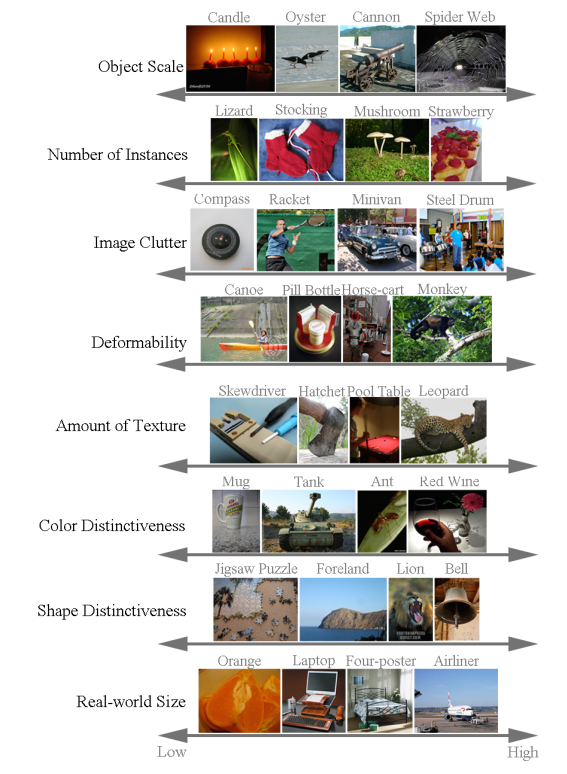
\includegraphics[width=0.5\textwidth]{../../sample_images/imnet_dimension}
    \caption{Eight diversity dimensions of the ImageNet dataset~\cite{imagenet_breakdown}}
    \label{fig:imnet_dimensions}
\end{figure}

\textbf{Class Balance}
The majority of classes contain 1300 examples, with some classes having fewer examples, as shown in
Figure~\ref{fig:imnet_dist}.

Based on this, we access the class distribution in the ImageNet dataset sufficiently balanced to not introduce bias, as
most classes contain 1300 images, and the classes with fewer examples are still represented by a reasonable number
of images, with all of them having more than 0.5 times the maximum number of samples.
Moreover, the most problematic group of classes with low sample numbers are multiple classes referring to specific dog breeds
like \textit{"black-and-tan coonhound"}, \textit{"otterhound"} and \textit{"English foxhound"} with 732,
738 and 754 samples, respectively.
As our goal for this project does not focus on generating image of different dog breeds, and just generating a
believable dog image would likely suffice, we think our position is further strengthened.

\begin{figure}[ht]
    \centering
    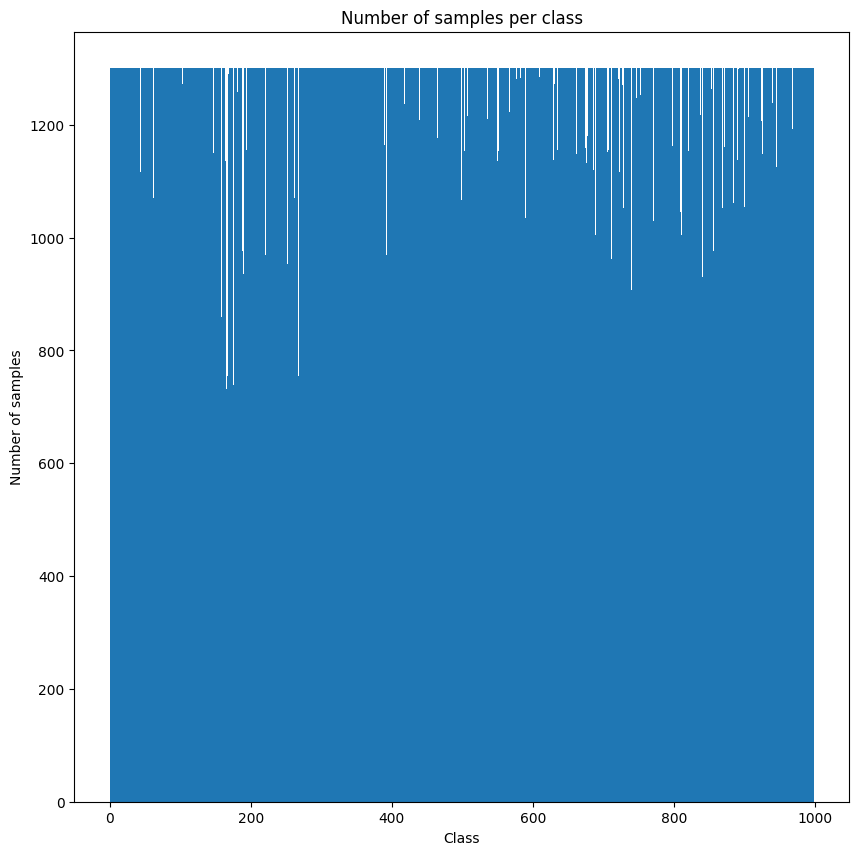
\includegraphics[width=0.5\textwidth]{../../sample_images/imagenet_dist}
    \caption{Distribution of images per class in the ImageNet dataset}
    \label{fig:imnet_dist}
\end{figure}

\textbf{Image Shapes}
Upon examining, we found that the images have highly irregular resolutions.
They belong to a range from 8x10 pixels to 9331x6530 pixels with a mean resolution of 471.7x404.7 pixels, as shown in
Figure~\ref{fig:imnet_sizes_err}.
The histogram in Figure~\ref{fig:imnet_sizes_hist} illustrates the distribution of image resolutions in the dataset.

As to be seen in figure~\ref{fig:optimal_resolution}, some images have a very irregular ratio, which imposes a challenge
for resizing.
Very small images do not contain enough information, which when upscaled, result in a blurry image (illustrated in
figure~\ref{fig:small_image}).

\subsubsection{Data Cleaning and Preprocessing}
In order to train the \ac{vq} on the ImageNet dataset, we will do the following preprocessing steps.

\begin{itemize}
    \item \textbf{Data Cleaning}
    Based on our knowledge from examining the image shapes, remove images with a resolution below 32px on any axis
    \item \textbf{Image Resizing}
    For training and testing, we resize all images to 128x128 pixels, similar to the paper.
    We use a composition of random cropping to extract a square image and resizing it to 128x128 pixels with
    the \texttt{v2.RandomResizedCrop} function from the TorchVision package.
    We set \texttt{scale=(0.2, 1.0)} and \texttt{ratio=1} to crop a square image with a sufficient area in
    relation to the original image, and enable anti-alias to reduce artifacts.
    \item \textbf{MinMax Normalizing}
    When input features have different scales, normalizing is a necessity for stable convergence.
    In the case of images, the pixel values represented by integers in the range of 0 to 255
    in each channel are already normalized to some degree.
    We scale them to floats in [0,1], further stabilizing the training process \cite{citationNeeded}.
    \item \textbf{Standardization:}
    Standardizing is a common step in machine learning and also often used for ImageNet, e.g.\ for training ResNet
    ~\cite{resnet}.
    It is also part of the standard TensorFlow and PyTorch preprocessing pipeline for ImageNet, and can protect
    against unwanted conditioning on image brightness. \\
    We standardize the images with the mean $\mu = (0.485, 0.456, 0.406)$ and standard deviation
    $\sigma = (0.229, 0.224, 0.225)$ of ImageNet for the three color channels, respectively.
\end{itemize}

Example images from ImageNet dataset after preprocessing are depicted in figure~\ref{fig:imnet_example_normalized}.

\subsection{CIFAR-10}\label{subsec:cifar-10}
CIFAR-10~\cite{cifar10} is another popular image classification dataset, as well as the larger version CIFAR-100.
CIFAR-10 consists of 60.000 32x32 pixel images, which are distributed over 10 classes.
The dataset is split into 50.000 training images and 10.000 test images.
The classes are mutually exclusive, so each image belongs to exactly one class.
The classes are: \textit{airplane, automobile, bird, cat, deer, dog, frog, horse, ship, truck}

The train set contains exactly 5000 images per class, while the test set contains 1000 images per class.
No image belongs to more than one class and there are no missing values or duplicates in the dataset.

\subsubsection{Preprocessing}
As the images in the CIFAR-10 dataset are already 32x32 pixels, we do not need to resize them.
Hence, we will only apply MinMax Normalizing and potentially Standardizing, same as for the ImageNet data.

Example images from the CIFAR-10 dataset are shown in figure~\ref{fig:cifar10_example_normalized}.
